% Submission working draft; page compression follows the narrative revision.
\begin{abstract}
LLM agents are known to be slow in rollouts. An agent completes a task one step at a time. At each step, it reasons and then chooses an action to execute. The next step and action cannot start until the previous one has finished.  
Speculative decoding accelerates the rollouts at the reason phase by drafting and verifying the inference tokens.
Recent works have also started to apply similar ideas at the action phase. These works use off-the-shelf models, usually large, to draft action proposals for target model to verify.
Large drafters match the target more often but take longer to propose, while small off-the-shelf models are fast but rarely make the same decision as the target.
We ask a more general question: what determines the end-to-end speedup of action speculation?
To answer it, we develop a latency framework for the speculative round. The framework compares what a round gains with what it costs. The gain depends on how well the drafter predicts the target and on how many steps the task can take before it ends. The cost comes from drafting, from waiting for target verification and from executing tools.
Guided by the framework, we introduce \textbf{LEAP} (\textbf{L}earning \textbf{E}fficient \textbf{A}ction \textbf{P}roposals) which keeps the drafter small and makes it accurate by training it on the target actions sequences.
With a small 0.6B model, LEAP agrees with the target on most decisions and makes agents up to 60\% faster in end-to-end wall clock time, with no systematic change in task success.
Across various datasets, target models and draft models, the framework accounts for most of the measured speedups.
We also show the draft model can be online trained with no prior trace collection and match the performance of offline training, making LEAP practical to deploy in the real world.
\end{abstract}

\section{Introduction}
An LLM agent solves a task through successive decisions, such as selecting a tool and supplying its
arguments. Each decision requires a full decode, often including reasoning, and later
decisions depend on earlier actions and observations. For our 32B target on one H100, a
$\tau^2$-bench task takes about three minutes, nearly all of it generation. Improving the latency of
this sequential loop matters even when its individual calls already use an efficient serving engine.

Speculative decoding reduces generation latency within a step. A cheap draft model proposes tokens
for an expensive target to verify~\citep{leviathan2023,chen2023}. Recent agent systems apply a similar
idea to whole actions. Their proposals come from off-the-shelf models, cheaper prompting configurations,
or the target itself~\citep{isp,dsp,specactions,spork,swyr}. These choices expose a tradeoff.
An untrained small model is cheap but may rarely agree with the target. A large self-draft agrees
more often but can spend much of the time that speculation was meant to save.

We ask what determines the end-to-end speedup of an action-speculation round. The draft proposes
up to $k$ actions, and the target verifies the resulting contexts concurrently. The round commits
the matching prefix and a target-generated correction or bonus unless the task ends.
Our latency framework compares the committed steps gained with the cost of proposing, waiting for
verification and executing tools. Efficient proposals must be likely to be accepted and cheap relative
to a target step. Acceptance alone does not determine speedup: a larger draft or the target itself
can be more accurate yet slower. Task endings further limit how many steps a round
can commit.

Guided by this framework, \textbf{LEAP} (Learning Efficient Action Proposals) keeps the draft small
and trains it to predict the target's canonical actions. Every target-authored commit supplies a
training pair, so supervision is a by-product of running the agent. Fine-tuning a LoRA adapter without
reproducing the reasoning text raises a 0.6B draft's agreement with Qwen3-32B from 2--25\% to 64--75\%
across our benchmarks (Table~\ref{tab:offline_main}). The draft proposes, the target decides, and both
share one GPU during inference.

The paper makes three contributions. First, the latency framework relates speedup to round gains
and costs. With measured hit rates and draft costs, its predictions are within 0.10 of measurement
on 19 of 21 configurations. Predictions using offline hit rates meet that threshold on 12 of 18
configurations; some use measured draft latency. Second, LEAP trains a tiny draft from the target's
own actions, either offline or online. Online inference starts near sequential per-step speed and
approaches the offline draft without a prior collection pass. Third, we evaluate four benchmarks,
two target families and three draft sizes on a shared GPU. The trained 0.6B gives 1.10--1.63\xx{}
whole-task speedup, up to about 60\% faster. Across 16 tool-benchmark comparisons, official task
success increases in eight, decreases in five and is unchanged in three, with differences of at
most three tasks. Planning termination counts are reported separately. Every committed action
passes the target-authorship audit. Figure~\ref{fig:loop} summarizes training and execution.

\begin{figure}[tbp]
\centering
\resizebox{\mainfigwidth}{!}{\begin{tikzpicture}[x=1cm,y=1cm,>=stealth,
 every node/.style={font=\fontsize{9}{10.5}\selectfont,inner sep=3pt},
 box/.style={draw=black!45,rounded corners=2pt,align=center,line width=.45pt},
 arr/.style={->,draw=black!65,line width=.65pt},
 tag/.style={font=\fontsize{8.5}{10}\selectfont,fill=white,inner sep=2pt}]
\useasboundingbox (-.1,.25) rectangle (14.3,6.55);
\node[anchor=west,font=\fontsize{9.5}{11}\selectfont\bfseries] at (0,6.25) {Train a small draft};
\node[box,fill=genfill,minimum width=2.8cm,minimum height=.8cm] (traces) at (1.5,5.4)
 {Frozen target\\training-task traces};
\node[box,fill=black!3,minimum width=3.25cm,minimum height=.8cm] (pairs) at (5.55,5.4)
 {Training pairs\\(context, target action)};
\node[box,fill=draftfill,minimum width=3.35cm,minimum height=.8cm] (train) at (10.1,5.4)
 {LoRA fine-tuning\\of a 0.6B draft};
\draw[arr] (traces) -- node[tag,above]{offline} (pairs);
\draw[arr] (pairs) -- (train);
\draw[arr,draw=draftline] (train.south) -- (10.1,4.45) -- node[tag,above]{updated draft adapter} (1.5,4.45) -- (1.5,3.28);
\node[anchor=west,font=\fontsize{9.5}{11}\selectfont\bfseries] at (3.95,3.98) {Verify concurrently with the target};
\node[box,fill=draftfill,minimum width=2.8cm,minimum height=1.35cm] (draft) at (1.5,2.6)
 {\textbf{Propose}\\$\hat a_1,\;\hat a_2$\\from context $s$};
\node[box,fill=genfill,minimum width=5.0cm,minimum height=.55cm] (v1) at (6.7,3.3)
 {$T(s)=\hat a_1$ \hspace{.6em} match};
\node[box,fill=genfill,minimum width=5.0cm,minimum height=.55cm] (v2) at (6.7,2.5)
 {$T(s,\hat a_1)=a_2\ne\hat a_2$ \hspace{.5em} mismatch};
\node[box,dashed,fill=black!2,text=black!55,minimum width=5.0cm,minimum height=.55cm] (v3) at (6.7,1.7)
 {$T(s,\hat a_1,\hat a_2)$ \hspace{.7em} cancel};
\draw[arr] (draft.east) -- (3.55,2.6) |- (v1.west);
\draw[arr] (3.55,2.6) |- (v2.west);
\draw[arr] (3.55,2.6) |- (v3.west);
\node[box,fill=savedfill,minimum width=3.15cm,minimum height=1.3cm] (commit) at (12.15,2.9)
 {\textbf{Commit}\\$\hat a_1,\;a_2$\\both target-authored};
\draw[arr] (v1.east) -- (9.85,3.3) |- ([yshift=6pt]commit.west);
\draw[arr] (v2.east) -- (9.85,2.5) |- ([yshift=-6pt]commit.west);
\draw[arr] (commit.south) -- (12.15,.65) -- node[tag,below]{append observations; next round} (1.5,.65) -- (draft.south);
\draw[arr,draw=savedline,dashed] (commit.east) -- (14.05,2.9) -- (14.05,6.25) --
 node[tag,above,text=savedline]{online: collect committed actions} (5.55,6.25) -- (pairs.north);
\end{tikzpicture}
}
\caption{\textbf{LEAP trains and uses an action draft.} Offline target traces or online commits supply
the training pairs. The adapter proposes actions; the target verifies their contexts concurrently.
In this $k=2$ example, one proposal matches and the target corrects the next. The remaining
verification is cancelled, and the two committed actions can become further training data.}
\label{fig:loop}
\end{figure}

\section{Related work}
\label{sec:related}
\paragraph{Token-level speculation.}
Speculative decoding preserves the target's token distribution while verifying draft tokens in
parallel~\citep{leviathan2023,chen2023}. Drafts may be separate models or prediction heads such as
Medusa and EAGLE~\citep{medusa,eagle}; DistillSpec and domain-adapted drafts train for higher
acceptance~\citep{distillspec,domaindraft}. Online speculative decoding updates a token draft using
deployment queries~\citep{osd}. OoO-Spec applies speculative decoding to tool calls~\citep{ooospec}. LEAP instead imitates canonical agent actions. 

\paragraph{Action and tool speculation.}
Interactive and Dynamic Speculative Planning use cheaper prompting configurations~\citep{isp,dsp};
Speculative Actions studies action-level verification and depth~\citep{specactions}; other systems
use untrained small models or modified target configurations~\citep{smc,spagent,dualspec}.
SPORK forks a probe from the target's state, while Speculate While You Reason trains a
self-speculation head jointly with the agent~\citep{spork,swyr}. We train a separate small draft with
the target frozen and measure both models together on one GPU.
Tool-latency methods launch predicted calls while generation continues~\citep{stc,paste,swm,aospec}.
They address a different cost from the sequential target-generation waits reduced by LEAP; our
proposals still pay tool-execution time. Additional comparisons are in App.~\ref{app:related}.

\section{Designing efficient action proposals}
\subsection{Propose, verify, commit}
\label{sec:problem}\label{sec:loop}
The context $s_i$ contains the instruction, tool schemas, and committed actions and
observations. The target greedily generates a canonical action $a_i=T(s_i)$; the draft predicts it
without reasoning. Actions must match after parsing and canonicalization, including tool names
and arguments; invalid proposals never match. Each synchronous round follows the propose--verify--commit pattern~\citep{specactions}
(Fig.~\ref{fig:loop}):
\begin{enumerate}
\item \textbf{Propose.} Generate up to $k$ actions, conditioned on earlier proposals and their
observations. Proposed tools execute in a copy of the environment.
\item \textbf{Verify.} The target generates actions on the resulting contexts, up to $k+1$,
concurrently on one shared GPU.
\item \textbf{Commit.} Consume verifications in prefix order. Commit the $A$ leading matches and
the target's correction or bonus, cancelling unused requests. Adopt accepted environment states
without executing their tools again.
\end{enumerate}
A round commits $A+1$ actions unless its accepted prefix completes the task, which leaves no
bonus. Proposing finishes before verification.

\begin{property}[target authorship]
\label{prop:exact}
Every committed action equals the target's verification output on the context in which that action
is committed.
\end{property}
The guarantee follows from matching before commit. Concurrent decoding can still change the target's
decisions, so trajectory identity and task outcomes are evaluated separately (App.~\ref{app:success}).

\subsection{A latency framework}
\label{sec:model}
The framework compares the steps gained with the time spent in a round, for any draft used in this loop.
Let $q_j=\Pr[A\ge j]$ include rounds that end before position $j$, and let $e$ be the probability that the
accepted prefix completes the task, which removes the bonus. The mean committed steps per round are
$c=1+\sum_{j=1}^{k}q_j-e$.

Let $t_{\mathrm{gen}}$ be the mean sequential target-generation time. Write $\beta t_{\mathrm{gen}}$
for the mean longest verification time actually awaited, and $D$ for mean proposing time per round
divided by $t_{\mathrm{gen}}$, including proposal-tool execution. With relative tool cost
$\tau=t_{\mathrm{tool}}/t_{\mathrm{gen}}$, let $f$ be the fraction of sequential steps executing a tool
and $g$ the mean number of target-executed tool steps per round. The speedup is approximately
\begin{equation}
 S\simeq\frac{c(1+f\tau)}{\beta+D+g\tau}
 \quad\xrightarrow{\;\tau\to0\;}\quad\frac{c}{\beta+D}.
 \label{eq:main:S}
\end{equation}
Accepted proposal tools are included in $D$ only once. This model assumes comparable work between
arms, small bookkeeping costs and cancellation of discarded verifications.

Efficient proposals are therefore likely to be accepted and cheap relative to a target step.
Pooled acceptance alone does not determine speedup: it omits rounds with no usable proposal and
does not encode task endings or proposing costs. Increasing depth can raise both commits
and round cost; the bounds and depth condition are in App.~\ref{app:model}.

\paragraph{Estimating the inputs.}
Estimate $c$ by evaluating the draft on held-out sequential target contexts and replaying the acceptance
rule and task endings. Estimate $\beta$ by replaying sequential timings with estimated hits and taking
each round's maximum awaited step time. Estimate $D$ from single-stream draft-latency
probes and the expected proposal count, plus proposal-tool costs (App.~\ref{app:predictor}).
Concurrency-dependent changes in target outputs and timing remain sources of prediction error.

\subsection{LEAP: training the draft}
\label{sec:train}
Guided by the framework, LEAP keeps the draft small and trains it on context--action pairs generated
by the frozen target. We fine-tune a LoRA adapter with cross-entropy on canonical action tokens,
discarding reasoning text. No target logits or human action labels are needed. The draft decodes
without reasoning and uses schema constraints on tool benchmarks; training settings are in
App.~\ref{app:detail:train}.

Only proposals conditioned on a fully matched prefix can be committed (Proposition~\ref{prop:commit}),
motivating supervised imitation on target traces. Property~\ref{prop:exact} also makes deployed
commits a source of online training pairs, without a separate collection pass.

\section{Experiments}
\label{sec:experiments}
\subsection{Setup and main results}
\label{sec:setup}\label{sec:results4}
We evaluate Qwen3-32B and Gemma-4-31B-it, each with trained Qwen3 drafts of 0.6B, 1.7B and 4B.
The whole pipeline is repeated for each target: its own sequential traces supply the training data.
Target and draft share one H100 during inference. Serving configurations are held fixed across
sizes within each benchmark; the Gemma target uses FP8 weights (App.~\ref{app:serving}).

We use four benchmarks. OpenAGI and TaskBench generate plans without executing tools~\citep{openagi,taskbench}.
$\tau^2$-bench uses the telecom domain in solo mode, with tools executed against its local backend;
BFCL uses multi-turn tasks and cloned tool environments~\citep{tau2bench,bfcl}.
Train/test splits are task-disjoint. Each task runs sequentially and speculatively on
the same service. We report the ratio of total sequential to speculative wall-clock. The main
speedup tables show the estimate $\pm$ one standard error (SE), computed as the standard deviation
of 10,000 task-level bootstrap ratios. Sequential and speculative times stay paired, and repeated
runs of a task remain together when resampled. Full 95\% intervals are retained in the appendix.

\begin{table}[htbp]
\centering\small\setlength{\tabcolsep}{6pt}\renewcommand{\arraystretch}{1.07}
\caption{\textbf{Whole-task speedup across benchmarks, targets and draft sizes.} Values are pooled
speedup factors $\pm$ one task-bootstrap SE (10,000 paired resamples); bold marks the largest rounded
point estimate per row. $k=3$ for planning and $k=2$ for tool benchmarks; test sizes are 63/60/40/60.
Qwen3 planning entries pool two runs. Full 95\% intervals and components: Table~\ref{tab:four}.}
\label{tab:main_results}
\begin{tabular}{llccc}
\toprule
Benchmark & Target & 0.6B & 1.7B & 4B \\
\midrule
OpenAGI & Qwen3-32B & $1.50\,\pm\,0.07$ & $\mathbf{1.55}\,\pm\,0.06$ & $1.46\,\pm\,0.08$ \\
 & Gemma-4-31B & $\mathbf{1.55}\,\pm\,0.11$ & $\mathbf{1.55}\,\pm\,0.11$ & $1.52\,\pm\,0.10$ \\
\addlinespace[3pt]
TaskBench & Qwen3-32B & $1.38\,\pm\,0.08$ & $\mathbf{1.47}\,\pm\,0.07$ & $1.36\,\pm\,0.08$ \\
 & Gemma-4-31B & $1.60\,\pm\,0.07$ & $\mathbf{1.68}\,\pm\,0.07$ & $1.62\,\pm\,0.06$ \\
\addlinespace[3pt]
$\tau^2$-bench & Qwen3-32B & $1.61\,\pm\,0.09$ & $\mathbf{1.63}\,\pm\,0.09$ & $1.56\,\pm\,0.08$ \\
 & Gemma-4-31B & $\mathbf{1.63}\,\pm\,0.07$ & $1.55\,\pm\,0.06$ & $1.55\,\pm\,0.06$ \\
\addlinespace[3pt]
BFCL & Qwen3-32B & $1.18\,\pm\,0.05$ & $1.28\,\pm\,0.04$ & $\mathbf{1.34}\,\pm\,0.07$ \\
 & Gemma-4-31B & $1.10\,\pm\,0.03$ & $1.12\,\pm\,0.03$ & $\mathbf{1.16}\,\pm\,0.04$ \\
\bottomrule
\end{tabular}
\end{table}


Table~\ref{tab:main_results} covers all three sizes and both targets. The trained 0.6B yields
1.18--1.61\xx{} with Qwen3 and 1.10--1.63\xx{} with Gemma. The benchmarks differ in the terms of
Eq.~\ref{eq:main:S}. OpenAGI accepts many proposals but its short tasks frequently remove the bonus.
$\tau^2$-bench has longer tasks and a cheap draft relative to its target generation time. BFCL
tasks are multi-turn conversations; a round cannot cross the end of a turn, and turns average only
2.6 steps, limiting commits per round.
Changing the target also changes the relative cost: Gemma's planning steps are longer, while its
tool-benchmark steps are shorter, so the same draft consumes a different fraction of a target step.

Every committed action passes the target-authorship audit. Across 16 comparisons on $\tau^2$-bench
and BFCL, official task success increases in eight, decreases in five, and is unchanged in three.
Differences are at most three tasks per comparison. The 12 planning-benchmark comparisons count
normal termination: three decrease and nine are unchanged (App.~\ref{app:success}). Trajectories
can still diverge. We report these outcomes separately from the per-action guarantee and retain
all tasks in the wall-clock estimator.

\subsection{Prediction: agreement with the target}
\label{sec:agreement}
We first examine how accurately a small draft predicts the target, which determines the
accepted-prefix contribution to a round's gain.
Table~\ref{tab:offline_main} compares draft agreement under a common evaluation setup. Training
substantially improves the small base. A reasoning-free target is a strong predictor on planning
tasks, but on $\tau^2$-bench it agrees on 42.5\% of contexts versus 63.7\% for the trained 0.6B.
Disabling reasoning can change the decision, so the target's size alone does not guarantee a better
action prediction. The reasoning-on target is also shown as a self-consistency reference.

\begin{table}[htbp]
\centering\small\setlength{\tabcolsep}{5pt}
\caption{\textbf{Offline action agreement (\%), Qwen3 target.} Estimate $\pm$ one task-bootstrap SE.
Draft types used in the cited work are evaluated here on common held-out contexts.
``Direct'' disables reasoning; ``reason'' enables it. BFCL includes turn ends.
Label sampling, repeated predictions and the bootstrap protocol are detailed in Table~\ref{tab:offline}.}
\label{tab:offline_main}
\begin{tabular*}{\linewidth}{@{\extracolsep{\fill}}lcccc@{}}
\toprule
Benchmark & 0.6B trained & 0.6B base & 32B direct & 32B reason \\
 & {\scriptsize (\textbf{LEAP})} & {\scriptsize\citep{smc}}
 & {\scriptsize\citep{isp,dsp}}
 & {\scriptsize\citep{spork,swyr}} \\
\midrule
OpenAGI & $75.0\,\pm\,3.1$ & $12.8\,\pm\,1.6$ & $76.6\,\pm\,2.3$ & $97.3\,\pm\,0.9$ \\
TaskBench & $75.2\,\pm\,3.0$ & $25.0\,\pm\,1.8$ & $84.8\,\pm\,2.2$ & $96.9\,\pm\,0.9$ \\
$\tau^2$-bench & $63.7\,\pm\,4.4$ & $8.0\,\pm\,1.1$ & $42.5\,\pm\,2.6$ & $65.0\,\pm\,4.0$ \\
BFCL & $66.7\,\pm\,6.0$ & $2.0\,\pm\,1.8$ & $62.6\,\pm\,3.7$ & $91.9\,\pm\,3.2$ \\
\bottomrule
\end{tabular*}
\end{table}


The SEs in Table~\ref{tab:offline_main} resample whole tasks and retain every context and repeated
prediction of each sampled task. Each replicate recomputes the context-weighted agreement, accounting
for dependence between decisions from the same trajectory. These SEs quantify task-sampling uncertainty
conditional on the evaluated models and runs; they do not quantify variation across training seeds.
BFCL has 99 contexts from ten tasks; its trained-draft SE is 6.0 percentage points. The $\tau^2$-bench
reasoning-on reference uses the per-context mode across three passes.

Task endings limit how often later proposals can be used (Sec.~\ref{sec:model}).
On OpenAGI, the second and third proposals are made in only 81\% and 62\% of rounds.
Among rounds that reach a position with the earlier proposals accepted, acceptance is about the
same as or higher than at the first position on every benchmark (Table~\ref{tab:agree}).

\paragraph{Supervision and objective.}
Table~\ref{tab:objective} tests learning the target's actions against benchmark gold supervision and
GRPO from the SFT draft. Gold-label training gives lower agreement on TaskBench and BFCL. The
comparison changes the training contexts as well as the labels: gold contexts follow gold actions,
and BFCL's target can group calls. The comparison therefore assesses the complete supervision source.
GRPO gives a small TaskBench gain and no BFCL gain, at substantially more
training cost; no variant exceeds the three-point agreement gain used to trigger an end-to-end run.

\begin{table}[htbp]
\centering\small
\caption{\textbf{Supervision and training objective.} Offline agreement (\%) for the Qwen3 target;
BFCL counts all decisions, including turn ends. Gold supervision also changes the training contexts.
No variant improves agreement by the three points required to trigger an end-to-end run.}
\label{tab:objective}
\begin{tabular}{llrr}
\toprule
 & & \multicolumn{2}{c}{offline agreement} \\
\cmidrule(lr){3-4}
objective & supervision & TaskBench & BFCL \\
\midrule
SFT on target actions (ours) & target's committed actions & 75.2 & 66.7 \\
SFT on gold labels & benchmark ground truth & 69.9 & 50.5 \\
GRPO from the SFT draft & exact-match reward & 77.1 & 65.7 \\
\bottomrule
\end{tabular}
\end{table}


\paragraph{Data and generalization.}
The OpenAGI recipe study separates the 40 test tasks whose action sequences also occur in training
from 23 with unseen sequences (Table~\ref{tab:recipe}). The default adapter obtains 82.2\% agreement
on the former and 64.5\% on the latter. Selecting epoch 7 by validation exact match raises overall
agreement from 75.0\% to 77.1\%, but the unseen score is 63.2\%. Full fine-tuning at epoch 7 gives
75.2\% overall, below the rank-64 adapter. Additional capacity or epochs therefore improve neither
subset uniformly in this study.

Using the same epoch-7 recipe with half or one quarter of the training pairs gives 72.0\% and
71.5\% overall agreement, versus 77.1\% with the full data. A few hundred pairs already supply
useful supervision, although performance depends on action-sequence overlap and the unseen score
is not monotone in data quantity. Cross-benchmark transfer is also limited: the TaskBench draft
reaches 23.3\% on OpenAGI and the OpenAGI draft 29.6\% on TaskBench, far below their in-benchmark
rates of about 75\% (Table~\ref{tab:transfer}). Most other transfers stay near the untrained base.
These results motivate workload-specific adapters and continued collection of the target's actions.
We retain action-only input because the target's reasoning is unavailable for later speculative
positions when the draft proposes them; full input and recipe studies are in App.~\ref{app:training}.

\subsection{Cost: when a more accurate draft is slower}
\label{sec:selfspec}\label{sec:training}
We next test whether extra agreement offsets the cost of proposing. The framework compares
the resulting gain in committed steps with the change in round time.

Figure~\ref{fig:curve} shows measured acceptance and drafting cost for the trained and untrained
0.6B drafts and the reasoning-disabled target. The untrained TaskBench draft produces no usable
proposal in 38\% of rounds; these rounds cost drafting time without entering the acceptance ratio
(Sec.~\ref{sec:model}).

\begin{figure}[tbp]
\centering
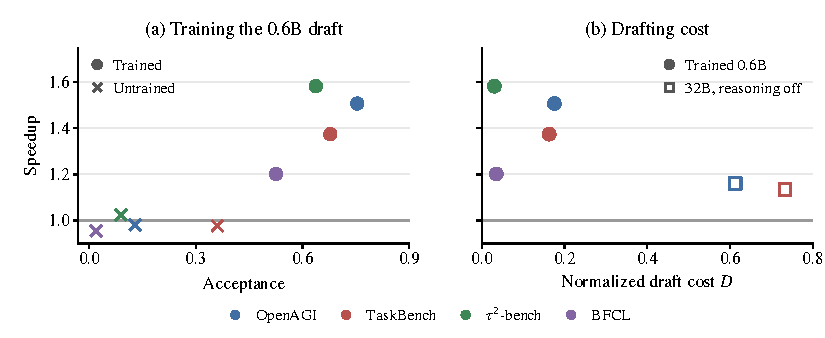
\includegraphics[width=\mainfigwidth]{figures/fig_curve.pdf}
\caption{\textbf{Measured acceptance and drafting cost, Qwen3 target.} (a) Trained and untrained
0.6B controls. Acceptance is the share of compared proposals that match the target. (b) Trained
0.6B on all four benchmarks, plus the reasoning-disabled target on the two planning benchmarks
where this control was run; $D$ is proposing time per round normalized by a target step. All points use the control runs of Table~\ref{tab:model}.}
\label{fig:curve}
\end{figure}

The planning controls use the target with reasoning disabled as the proposer in our same
propose--verify--commit loop. Their live acceptance is comparable to or above the trained draft's,
yet Qwen3 self-drafting gives only 1.16\xx{} and 1.13\xx{} on OpenAGI and TaskBench
(Table~\ref{tab:model}). Each proposal costs $3.3$--$4.0\times$ as much, raising the normalized draft
term from 0.16--0.18 to 0.61--0.73. With Gemma's longer planning steps, self-drafting instead reaches
1.48\xx{} and 1.54\xx{}: drafting cost is smaller relative to a target step. These measurements
illustrate why acceptance and relative cost must be considered together.

\paragraph{Draft size.}
Figure~\ref{fig:size} shows the draft-size ablation. On Qwen3 planning tasks, agreement generally
increases with size, but a 4B draft is slower than 1.7B and returns to about the 0.6B speedup. Its
per-round cost grows from 0.16--0.17 to 0.28--0.29 target steps, offsetting the extra commits.
On BFCL, greater agreement carries through to higher speedup because drafting is cheap relative to
the target step. On $\tau^2$-bench the three sizes' 95\% intervals overlap (Table~\ref{tab:four}). Gemma changes this balance
again: its shorter tool-benchmark generations increase the relative draft cost, and its 0.6B draft
is fastest on $\tau^2$-bench (Table~\ref{tab:main_results}).

\begin{figure}[tbp]
\centering
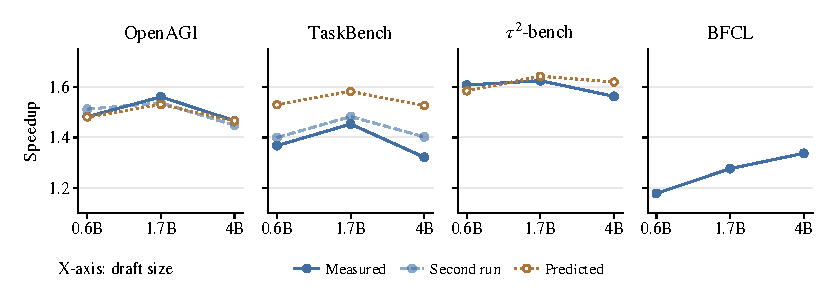
\includegraphics[width=\mainfigwidth]{figures/fig_size.pdf}
\caption{\textbf{Draft-size ablation, Qwen3 target.} Measured speedup, independent planning repeats,
and the predictions used in Fig.~\ref{fig:pred}b. BFCL has one measured size study and no offline-hit
prediction. Agreement and cost values are in Table~\ref{tab:size}; pooled results are in
Table~\ref{tab:main_results}.}
\label{fig:size}
\end{figure}

The cost decomposition makes this comparison quantitative. In the generation-dominated regime,
the model compares two draft configurations through
\begin{equation}
 \frac{S_B}{S_A}\simeq
 \frac{c_B/c_A}{(\beta_B+D_B)/(\beta_A+D_A)}. \label{eq:main:size_ratio}
\end{equation}
For the measured Qwen3 components, moving from 0.6B to 4B raises commits per round by a factor
of 1.09--1.10 on the planning benchmarks but raises round cost by 1.12, explaining the loss in
speedup. On BFCL the corresponding factors are 1.16 and 1.03, so the larger draft pays off.
On $\tau^2$-bench both ratios are within 0.02 of one. These are explanations using measured
components; predictive comparisons use estimated components in the same ratio. Their resolution
depends on the relative input errors, particularly when expected speedups differ by only a few
hundredths. The full confidence intervals and repeated planning runs provide the relevant empirical
context for these point-estimate comparisons.

The 0.6B draft is within 0.1\xx{} of the fastest size in seven of eight benchmark--target pairs.
For practitioners, we recommend starting with a trained 0.6B draft and $k{=}1$.
The main runs use the benchmark settings in Table~\ref{tab:main_results}; depth studies and their
uncertainty are reported in Table~\ref{tab:model}. The recommendation prioritizes low drafting and
training cost.

\noindent
\begin{minipage}[t]{0.56\linewidth}
\vspace{0pt}
\textbf{Tool latency.}
Adding 2 or 5 seconds to every executed tool step in both arms tests the tool terms. At 5 seconds,
measured speedup falls to 1.20\xx{} on $\tau^2$-bench and 1.02\xx{} on BFCL; trace-replay $\beta$
predicts 1.17\xx{} and 1.04\xx{} using measured hit rates and proposing costs (Table~\ref{tab:tool}).
Agreement changes little, but proposals pay tool latency while rolling out. The normalized proposing
cost grows from 0.03 to 0.31 and 0.74 on $\tau^2$-bench, and from 0.04 to 0.23 and 0.50 on BFCL.
On BFCL, turn ends execute no tool, so $f=0.62$ and $g=0.44$--$0.45$ (App.~\ref{app:predictor}).
\end{minipage}\hfill
\begin{minipage}[t]{0.41\linewidth}
\vspace{0pt}
\centering\footnotesize\setlength{\tabcolsep}{3pt}
\captionsetup{type=table}
\caption{\textbf{Tool-delay speedups.} Qwen3, trained 0.6B, $k=2$.}
\label{tab:tool}
\begin{tabular}{lrrr}
\toprule
 & Delay (s) & Pred. & Meas. \\
\midrule
$\tau^2$-bench & 0 & 1.58 & 1.58 \\
               & 2 & 1.36 & 1.41 \\
               & 5 & 1.17 & 1.20 \\
\midrule
BFCL           & 0 & 1.30 & 1.20 \\
               & 2 & 1.15 & 1.07 \\
               & 5 & 1.04 & 1.02 \\
\bottomrule
\end{tabular}

\end{minipage}
\par\medskip
A round also pays for the target's own tool action, while accepted proposal states are adopted.
These costs account for the loss of speedup despite nearly unchanged hit rates. The four added-delay
predictions are within about 0.08\xx{} of measurement; using the measured verification wait reduces
the residual to about 0.02\xx{}. This diagnostic supports the tool-cost accounting while identifying
wait estimation as a remaining error source.

\subsection{Checking the latency framework}
\label{sec:validation}
Finally, we test the framework's combined accounting of round gains and costs against measured speedup.
We first validate the accounting with the run's measured hit rates and draft cost, while predicting
$\beta$ from its sequential timing trace. Across 21 configurations spanning depths, untrained
drafts, self-drafting and added tool latency, predicted speedup is within 0.05\xx{} on 14 and
within 0.10\xx{} on 19 (Fig.~\ref{fig:pred}a). Component checks and full inputs are in
Fig.~\ref{fig:components} and Table~\ref{tab:model}.

\begin{figure}[tbp]
\centering
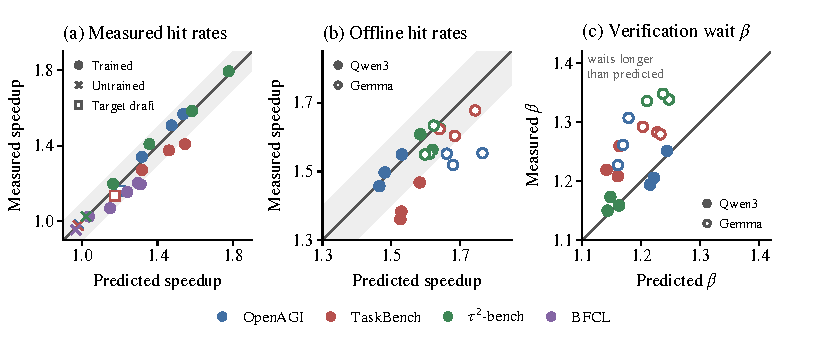
\includegraphics[width=\linewidth]{figures/fig_pred_vs_meas.pdf}
\caption{\textbf{Predicted versus measured speedup and verification wait.} (a) 21 Qwen3 controls with measured hit rates
and draft cost. (b) Nine size-study configurations per target, using offline hit rates and trace-replay
$\beta$; draft timing sources are in Table~\ref{tab:prediction_inputs}. (c) Verification wait $\beta$ for the
points of (b): the trace-replay prediction used in (b) against the measured value. Points above the
diagonal waited longer than predicted, which raises the predicted speedup. Axes have equal scales within
each panel; shading marks $\pm0.10$ in (a) and (b).}
\label{fig:pred}
\end{figure}

We then replace live hit rates with the draft's predictions on held-out sequential contexts and
replay the commitment rules without live acceptance measurements. In the Qwen3 control runs, offline draft-latency probes
and trace-replay $\beta$ predict 1.48, 1.56 and 1.59\xx{} on OpenAGI, TaskBench and $\tau^2$-bench,
against 1.51, 1.37 and 1.58\xx{} measured. Figure~\ref{fig:pred}b
applies the same replay to all three draft sizes in the serving configurations of Table~\ref{tab:main_results},
giving nine points per target. The 1.7B and 4B Qwen3 planning drafts and the larger Gemma drafts use
measured per-proposal latency, so these predictions are conditional on that cost. Twelve of the eighteen
size-study predictions are within 0.10\xx{}. The control and size studies use their respective serving
configurations; their 0.6B measurements need not coincide.

The errors differ by target. The trace replay underestimates the verification wait $\beta$ on every
Gemma configuration, by 0.05--0.13, and on Qwen3 TaskBench, by 0.05--0.10; on Qwen3 OpenAGI and
$\tau^2$-bench it is within 0.03 (Fig.~\ref{fig:pred}c). A lower $\beta$ raises the predicted speedup:
all six points that miss by more than 0.10 in (b) have an underestimated $\beta$. The cause of this
gap is not established. On Qwen3 TaskBench the replay also overpredicts the first-position hit rate
(0.73 versus 0.66 in the control run), because live trajectories depart from the sequential trace more
often than on OpenAGI. On Gemma $\tau^2$-bench, the replay's lower hit rates offset the $\beta$ gap, so a
small total speedup error can reflect cancellation between input errors. These effects limit reliable
ranking of nearby configurations. BFCL is not in (b) or (c) because it has no offline-hit prediction
(App.~\ref{app:detail:validation}).

\FloatBarrier
\subsection{Learning the draft online}
\label{sec:online}
The separate trace-collection pass is optional: committed actions are target-authored even when the
draft is initially untrained. We start the speculative system with the 0.6B base and process the
training tasks in batches: 25 tasks on OpenAGI and 10 on $\tau^2$-bench. After each batch, an adapter
is trained on all commits so far on a second GPU and loaded into the draft server. Batch $b$ uses
only the adapter trained on earlier batches. A continual variant instead updates the previous
adapter on the new batch plus an equal-size sample of earlier pairs.

\begin{figure}[htbp]
\centering
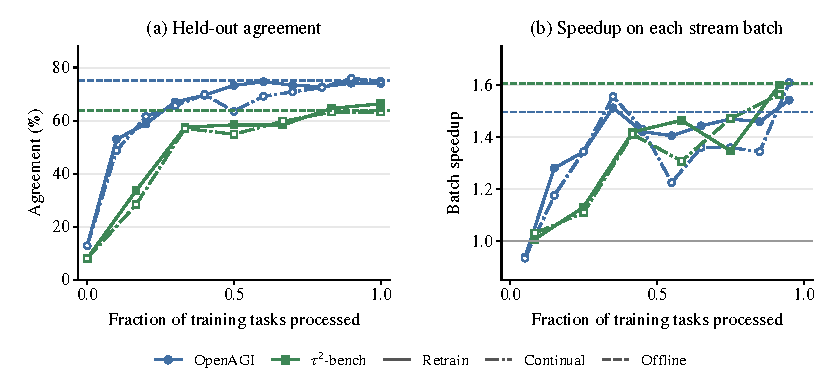
\includegraphics[width=\mainfigwidth]{figures/fig_online.pdf}
\caption{\textbf{Learning online, Qwen3 target.} (a) Held-out agreement after each adapter update.
(b) Speedup on each stream batch, placed at the batch midpoint: sequential time per step over
speculative time per committed step. Dashed lines are offline drafts. Each batch uses an adapter
trained on earlier tasks. Training time is reported separately; final test results are in
Table~\ref{tab:online_final}.}
\label{fig:online}
\end{figure}

Agreement grows rapidly (Fig.~\ref{fig:online}a). On OpenAGI, retraining reaches 53\% after 25 tasks,
67\% after 75, and 74.0\% after 250, against the offline draft's 75.0\%. Its batch speedup rises
from 0.94\xx{} initially to 1.4--1.5\xx{} from the fourth batch. On $\tau^2$-bench, agreement rises
from 8.0\% to 66.4\%, versus 63.7\% offline, and the batch speedup rises from 1.01\xx{} to 1.4\xx{}
after 20 tasks and 1.60\xx{} in the last batch (Fig.~\ref{fig:online}b). The final adapters attain
similar test speedups to the offline drafts (Table~\ref{tab:online_final}).

\begin{table}[htbp]
\centering\small\setlength{\tabcolsep}{7pt}
\caption{\textbf{Final online adapters on the test split, Qwen3 target.} Whole-task inference
speedup $\pm$ one task-bootstrap SE, using trained 0.6B drafts with matched offline and online serving settings. Training time is separate; 95\% intervals are in Table~\ref{tab:online_final_ci}.}
\label{tab:online_final}
\begin{tabular}{lccc}
\toprule
Benchmark & Offline & Online: retrain & Online: continual \\
\midrule
OpenAGI & $1.51\,\pm\,0.07$ & $1.47\,\pm\,0.08$ & $1.51\,\pm\,0.06$ \\
$\tau^2$-bench & $1.61\,\pm\,0.09$ & $1.61\,\pm\,0.10$ & $1.63\,\pm\,0.10$ \\
\bottomrule
\end{tabular}
\end{table}


Retraining on the growing buffer costs 27--73 seconds per update on OpenAGI and 3--18 minutes on
$\tau^2$-bench. Continual updates take about 22 seconds and 3--6 minutes respectively. They reach
similar endpoints, though OpenAGI dips once before recovering. Update times are reported separately
from inference speedups.
Version-by-version agreement and update timings are in App.~\ref{app:online}.

\section{Conclusion and Limitations}
\label{sec:conclusion}
We asked what determines end-to-end speedup in action speculation. The latency framework compares
the committed steps gained with proposing, verification and tool costs. It identifies the design
goal of proposals that are likely to be accepted and cheap relative to a target step. LEAP meets
this goal by training a tiny draft on the frozen target's actions. Across four benchmarks and two
target families, the trained 0.6B gives 1.10--1.63\xx{} whole-task speedup on one shared GPU.
The same supervision is available during deployment, allowing online training without a prior
trace-collection pass.

We evaluate two target families across various benchmarks, using local
simulated tool backends. The framework covers synchronous proposing followed by exact-match
verification, with target contexts verified concurrently on one GPU. It does not cover asynchronous
draft run-ahead, semantic verification or methods that hide tool latency through overlap.
The loop trades target compute for latency: verification can issue up to
$k+1$ requests per round, and $\tau^2$-bench uses 1.16\xx{} the sequential completion tokens in
the measured control. Slow tools reduce its benefit because proposing pays their execution cost.
Concurrent decoding can change whole trajectories despite target authorship. The predictor assumes
comparable work and transfer of sequential timing to concurrent requests; these approximations and
the bootstrap intervals limit close configuration comparisons. Online training could consume additional
resources depending on the actual setup.
\label{main:text_end}
